% This LaTeX was auto-generated from MATLAB code.
% To make changes, update the MATLAB code and export to LaTeX again.

\documentclass{article}

\usepackage[utf8]{inputenc}
\usepackage[T1]{fontenc}
\usepackage{lmodern}
\usepackage{graphicx}
\usepackage{color}
\usepackage{hyperref}
\usepackage{amsmath}
\usepackage{amsfonts}
\usepackage{epstopdf}
\usepackage[table]{xcolor}
\usepackage{matlab}

\sloppy
\epstopdfsetup{outdir=./}
\graphicspath{ {./hofstadterbutterfly_images/} }

\begin{document}

\label{H_F310D61F}
\matlabheading{Hodstadter's butterfly}


\vspace{1em}
\matlabheadingthree{Tight binding Hamiltonian with magnetic field}

\begin{par}
\begin{flushleft}
The tight binding Hamiltonian with Peierls substitution can be generated with \texttt{normalMetalRectangularCell(in)}.
\end{flushleft}
\end{par}

\begin{par}
\begin{flushleft}
\texttt{in }is a structure consisting of elements:
\end{flushleft}
\end{par}

\begin{par}
\begin{flushleft}
\texttt{Nx, Ny - System lengths}
\end{flushleft}
\end{par}

\begin{par}
\begin{flushleft}
\texttt{chemPot - Chemical potential}
\end{flushleft}
\end{par}

\begin{par}
\begin{flushleft}
\texttt{hopInt - Hopping integral}
\end{flushleft}
\end{par}

\begin{par}
\begin{flushleft}
\texttt{b - Magnetic field strength scaled with }$2\pi$
\end{flushleft}
\end{par}

\begin{par}
\begin{flushleft}
\texttt{impurityArray - An array of potential impurities, major order along x}
\end{flushleft}
\end{par}


\vspace{1em}
\begin{par}
\begin{flushleft}
Generate eigenvalues across different values of magnetic field \texttt{b} in a for-loop for different Hamiltonian with \texttt{testRectangular.m}.
\end{flushleft}
\end{par}

\begin{par}
\begin{flushleft}
Plotting eigenenergy against normalized magnetic field strength alpha gives us the Hofstadter's butterfly.
\end{flushleft}
\end{par}

\begin{par}
\begin{flushleft}
Plot source code:
\end{flushleft}
\end{par}

\begin{matlabcode}
run("hofBFPlot.m")
\end{matlabcode}
\begin{center}
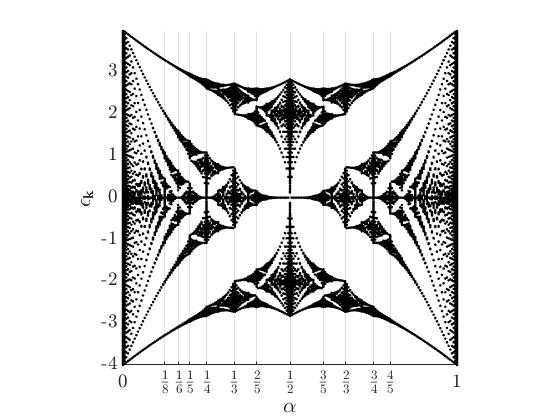
\includegraphics[width=\maxwidth{56.196688409433015em}]{figure_0.png}
\end{center}

\end{document}
